\documentclass{article}

\usepackage{lipsum}
\usepackage[margin=1.5in]{geometry}
\usepackage{titlesec}
\usepackage{graphicx}
\usepackage{amsmath}

\usepackage{mathtools, amssymb, nccmath}
\usepackage{bigstrut, changepage, lipsum}
\usepackage{mathtools}

\newcommand{\code}{\texttt}
\newcommand{\norm}[1]{\left\lVert#1\right\rVert}

\usepackage{siunitx} % Required for alignment


% Specify images directory
\graphicspath{ {./report-images/} }

% Header and Footer stuff
\usepackage{fancyhdr}
\pagestyle{fancy}
\fancyhead{}
\fancyfoot{}
\fancyfoot[R]{ \thepage\ }
\renewcommand{\headrulewidth}{0pt}
\renewcommand{\footrulewidth}{0pt}
\newcommand{\sectionbreak}{\clearpage}
\setlength{\parindent}{0pt}

%

\begin{document}

%----------------------------------------------------------------------------------------
%	TITLE PAGE
%----------------------------------------------------------------------------------------

\begin{titlepage} % Suppresses displaying the page number on the title page and the subsequent page counts as page 1
	\newcommand{\HRule}{\rule{\linewidth}{0.5mm}}% Defines a new command for horizontal lines, change thickness here
	
	\center % Centre everything on the page
	
	%------------------------------------------------
	%	Headings
	%------------------------------------------------
	
	\textsc{\Large Basic orthogonal and periodic functions}\\[0.5cm] % Major heading such as course name
	
	\textsc{\large Exercise 3}\\[0.5cm] % Minor heading such as course title
	
	%------------------------------------------------
	%	Title
	%------------------------------------------------
	
	\HRule\\[0.6cm]
	
	{\huge\bfseries Least-squares Approximation of cos(2x) and cos(4x) Using Chebyshev Polynomials}\\[0.25cm] % Title of your document
	
	\HRule\\[1.5cm]
	
	%------------------------------------------------
	%	Author(s)
	%------------------------------------------------
	
	\begin{minipage}{0.4\textwidth}
		\begin{flushleft}
			\large
			\textit{Author}\\
			\textsc{Cesare De Cal} % Your name
		\end{flushleft}
	\end{minipage}
	~
	\begin{minipage}{0.4\textwidth}
		\begin{flushright}
			\large
			\textit{Professor}\\
			\textsc{Annie Cuyt}\\ % Supervisor's name
			[0.25cm]
			\textit{Assistant Professor}\\
			\textsc{Ferre Knaepkens} % Supervisor's name

		\end{flushright}
	\end{minipage}
		
	\vfill\vfill\vfill
	
	{\large\today}
		
	\vfill
	
\end{titlepage}

%----------------------------------------------- Introduction ------------------------------------------------------
\section{Introduction}\label{sec:intro}
This exercise asks to compute the Chebyshev approximation
$$t(x)=\sum^n_{j=0}{a_jT_j(x)}$$

for the functions $f(x)=\cos(2x)$ and $f(x)=cos(4x)$ over the interval $[-\pi,\pi]$ for $n = 6$ and then plot the original functions with the approximations and draw conclusions on the results.\\

As we've seen in class, Chebyshev polynomials are a set of orthogonal polynomials that can be used to approximate to a least squares fit. For this exercise, I'll first compute the roots of the polynomial (also called Chebyshev nodes), then calculate its coefficients for both the functions. Finally, I'll calculate the y values of the approximation to see how well it approximates the original function. During this process, I'll make sure to choose the correct data points and the correct number of data points to exploit the properties of these basis functions.

%---------------------------------- Tools ---------------------------------------------------------------------------
\section{Tools}
To solve this problem, I've used MATLAB as requested by the exercise. To make the computation more efficient, I wrote my own function which calculates the Chebyshev polynomial instead of using the built-in MATLAB function $\code{chebyshevT}$ which was noticeably slower. Writing my own function was just a matter of using the compact closed-form expression for the Chebyshev polynomials:

$$T_i(x)=\cos{(i\arccos(x))}$$ 

Built-in MATLAB functions have been used such as $\code{cos(x)}$ and $\code{acos(x)}$ to calculate the cosine and the inverse cosine function. $\code{linspace(start, end, nrOfPoints)}$ was used to create an array of equidistant points for plotting. The functions $\code{plot(x, y)}$, $\code{legend()}$, $\code{axis([xmin xmax ymin ymax])}$, $\code{ylabel(label)}$, and $\code{xlabel(label)}$ were also used for plotting.

\section{Computation}
Given $n=6$, I first calculate the nodes of the Chebyshev polynomial by using the formula:

$$x_j=\cos \Big( \frac{2j-1}{2n}\pi \Big), j=1,\dots,n+1$$

The resulting zeros are:

$$
\begin{bmatrix} 
9.749279121818236e-01\\
7.818314824680298e-01\\
4.338837391175582e-01\\
6.123233995736766e-17\\
-4.338837391175581e-01\\
-7.818314824680295e-01\\
-9.749279121818237e-01\\
\end{bmatrix}
$$

Let's first analyze the function $\cos(2x)$. We've seen in class we can calculate the coefficients with the formula given by:

$$c_j=\frac{2}{N}\sum_{k=0}^{n}f(x_j)T_j(x_k)$$

To better exploit the properties of Chebyshev polynomials, I rescale the interval from $[-\pi,\pi]$ to $[-1,1]$. This is done in the function calculation $f(x_j)$ by multiplying the argument by $\pi$. I find the following coefficients:

$$
\begin{bmatrix} 
4.407675118300712e-01\\
3.489272363107635e-16\\
5.739892333362830e-01\\
-2.537652627714643e-16\\
6.516380108719009e-01\\
-1.554312234475219e-15\\
-7.019674665493458e-01\\
\end{bmatrix}
$$

The polynomial for the first function $\cos{2x}$ looks like this:

\begin{equation}
  \begin{array}{l}
    t(x) = 4.407675118300712e-01 \times T_0(x)+ 3.489272363107635e-16 \times T_1(x) + \\ 
    5.739892333362830e-01 \times T_2(x) + \dots -7.019674665493458e-01 \times T_6(x)
  \end{array}
\end{equation}

To plot these coefficients in the graph, I need to calculate their associated y values:

$$
\begin{bmatrix}
9.876173836808355e-01\\
1.986723718905843e-01\\
-9.149466098687946e-01\\
9.999999999999993e-01\\
-9.149466098687926e-01\\
1.986723718905768e-01\\
9.876173836808371e-01\\
\end{bmatrix}
$$

Calculating the coefficients for the $\cos(4x)$ function now only requires minor changes in the code. The following are the coefficients of the polynomial:
$$
\begin{bmatrix} 
6.879841220704104e-01\\
2.537652627714643e-16\\
-1.535576743556636e-01\\
-1.459150260935920e-15\\
1.012919200612446e+00\\
-1.094362695701940e-15\\
5.104689360033142e-01
\end{bmatrix}
$$

The polynomial for the second function $\cos{4x}$ looks like this:

\begin{equation}
  \begin{array}{l}
    t(x) = 6.879841220704104e-01 \times T_0(x) + 2.537652627714643e-16 \times T_1(x) \\ 
    -1.535576743556636e-01 \times T_2(x) + \dots + 5.104689360033142e-01 \times T_6(x)
  \end{array}
\end{equation}

The associated y values for the given roots are the following:

$$
\begin{bmatrix} 
9.507761930971577e-01\\
-9.210585772947382e-01\\
6.742545978208001e-01\\
1.000000000000000e+00\\
6.742545978207990e-01\\
-9.210585772947411e-01\\
9.507761930971639e-01\\
\end{bmatrix}
$$

In order to properly calculate the associated y values, I had to subtract half of the first coefficient from the calculation. This is done because the formula I used to calculate the coefficients isn't correct for the first coefficient. The plots for both functions have been added to the next section.\\

\section{Plots}
Function $\cos(2x)$:\\
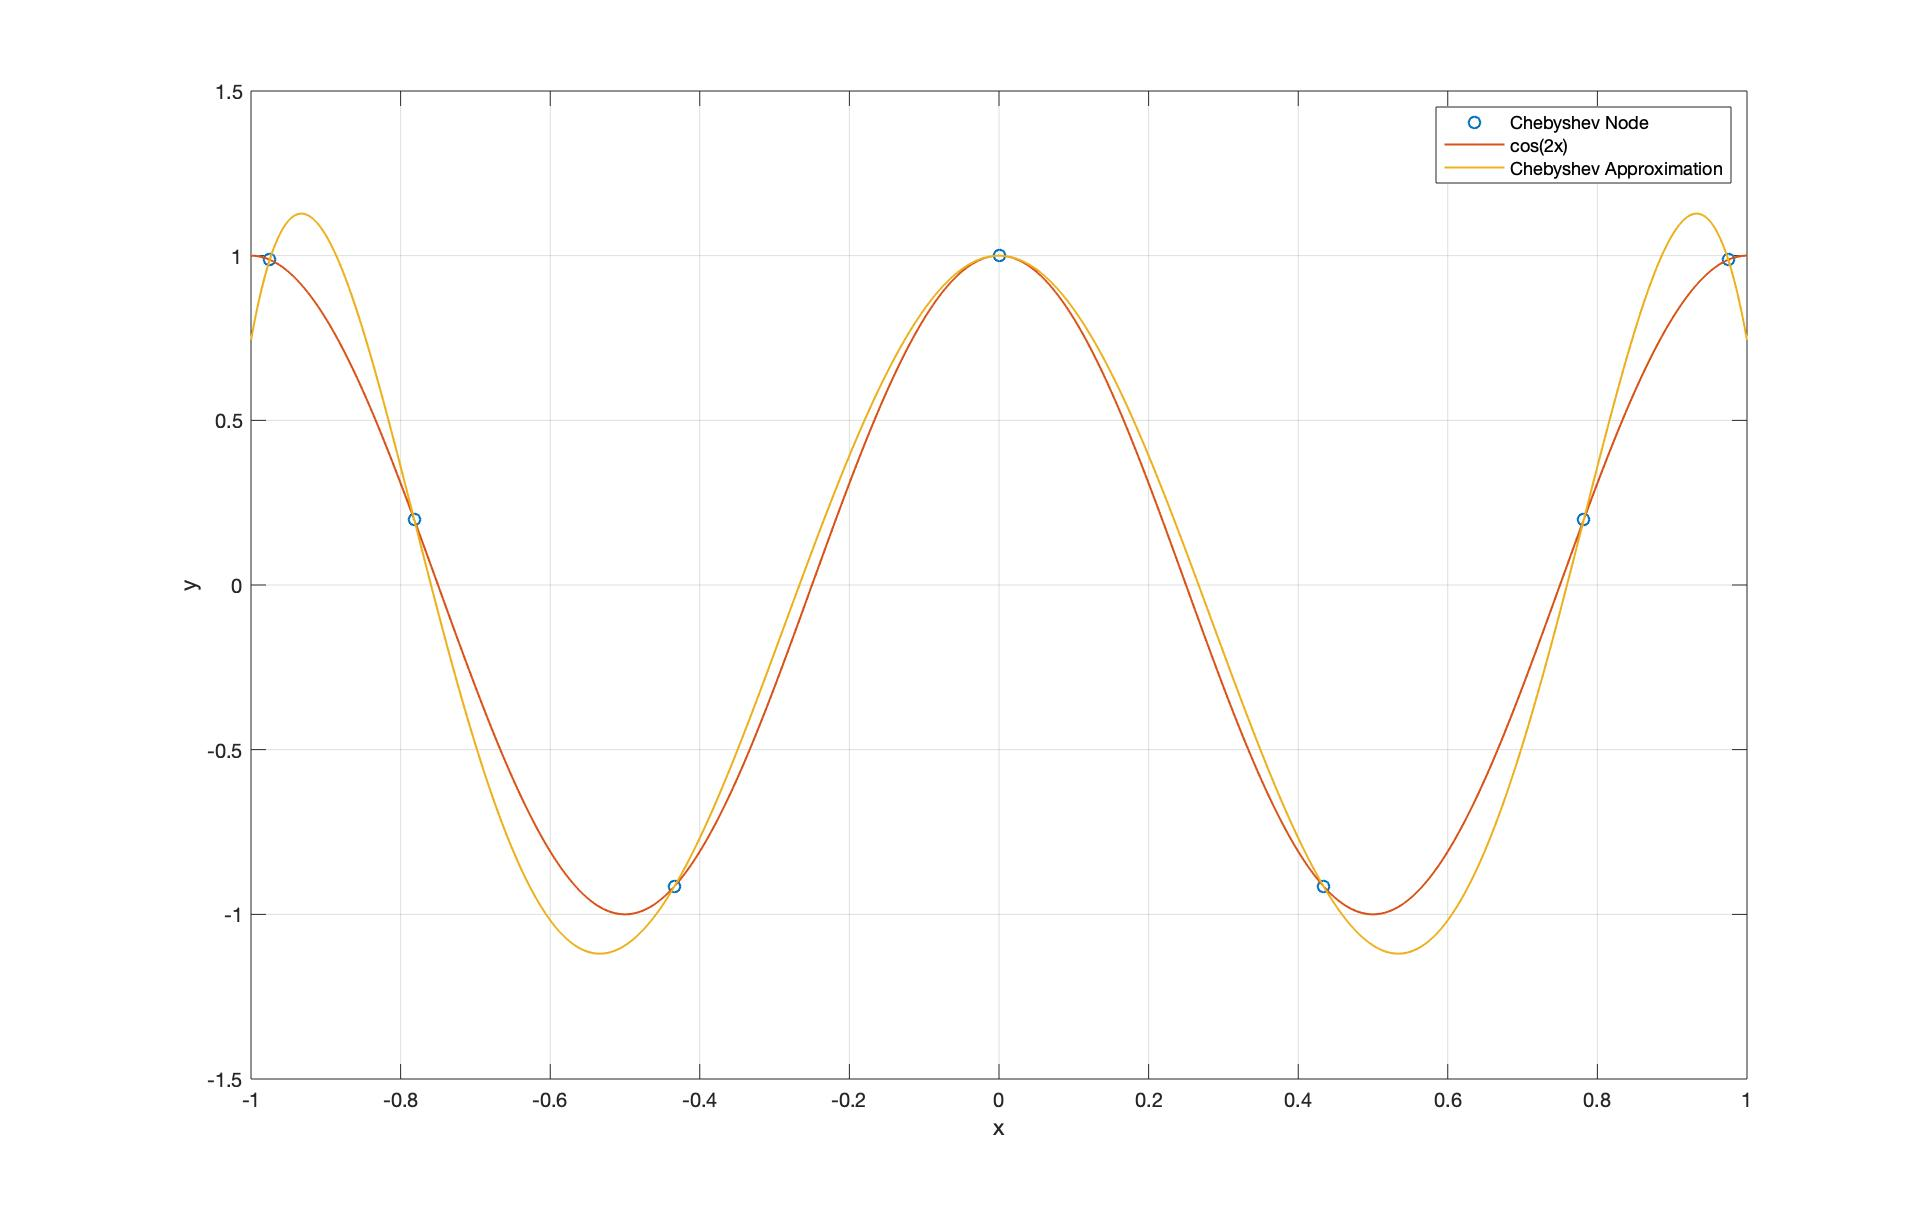
\includegraphics[width=\textwidth,height=\textheight,keepaspectratio]{cos2x.jpg}\\
Function $\cos(4x)$:\\
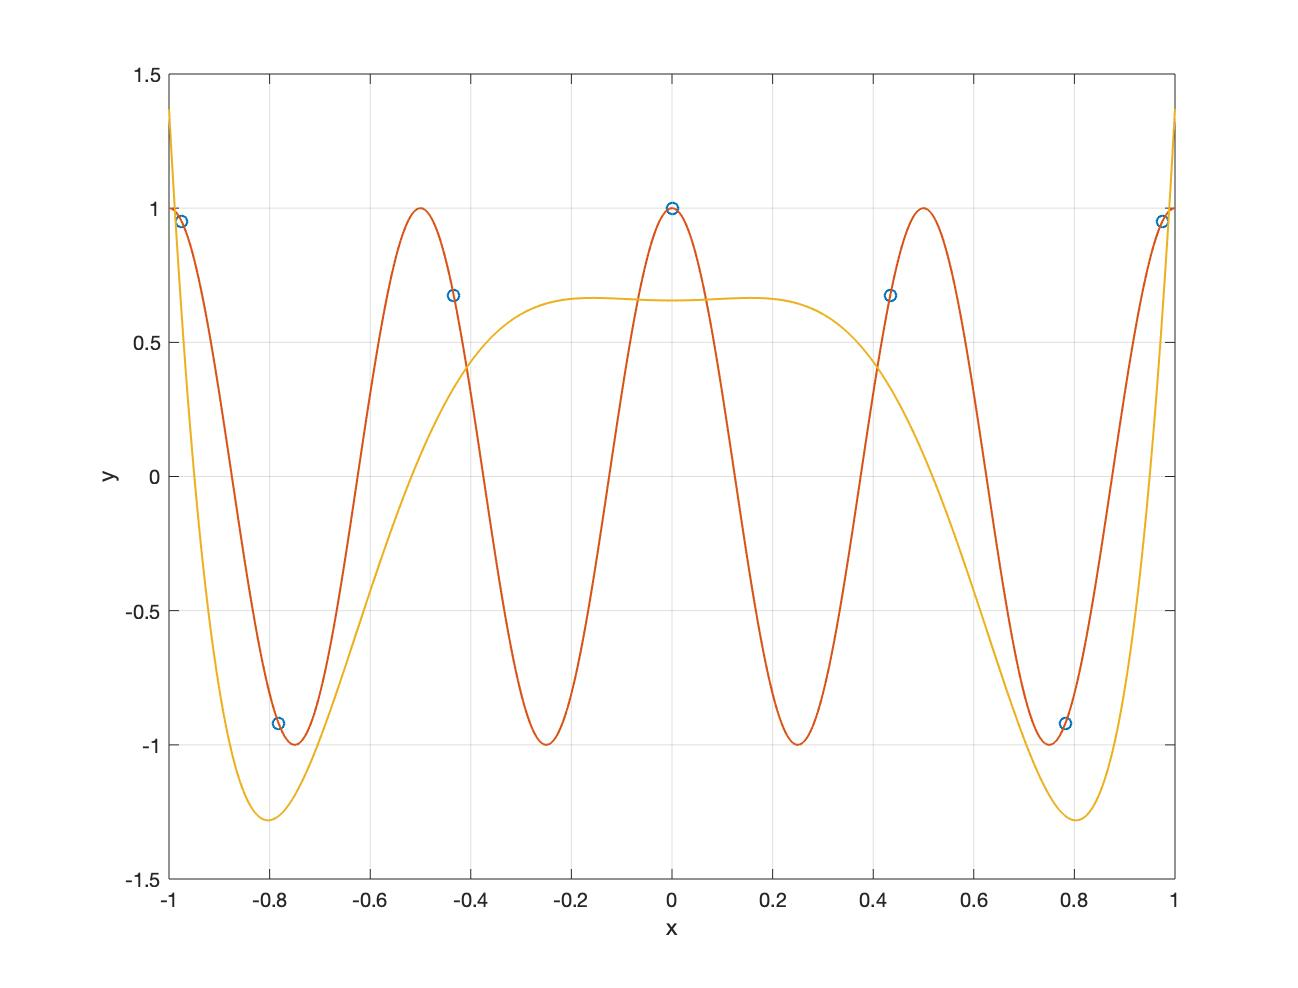
\includegraphics[width=\textwidth,height=\textheight,keepaspectratio]{cos4x.jpg}
\section{Observations}
I first calculated the zeros of the polynomial so I could use them as nodes in polynomial interpolation because the resulting interpolation polynomial minimizes the effect of Runge's phenomenon. The functions, however, still display a little bit of Runge's phenomenon. \\

The Chebyshev approximation for the function $\cos(2x)$ is pretty accurate, whereas the approximation for $\cos(4x)$ not so much as it doesn't take into account some of the spikes of the original function.

\end{document}